% Images can be scaled only using absolute width or height
% A4 paper width is 21cm
% borders in 2024 template are 2.54cm
% So \textwidth is set to 21 - 2*2.54 = 15.92cm
% You can change them in header.tex

Sed ut perspiciatis unde omnis iste natus error sit voluptatem accusantium doloremque\refcite{minsky2017perceptrons} laudantium.

With a different Footnote~\footnote{Another footnote}, bold text \textbf{emphasized text} and a citation\cite{einstein2013principle}. Let's add some math $y = mx + c$ and italics \textit{highlighted}. And also itemize and lists:
\begin{itemize}
	\item Item A
	\item Item B
\end{itemize}
\begin{enumerate}
	\item Item Alpha
	\item Item Beta
\end{enumerate}

You can use the provided commands \textit{textwidth}, \textit{threequartertextwidth}, \textit{halftextwidth}, \textit{onequartertextwidth} to scale images.
Or you can use explicit size, knowing that \textit{textwidth} is 15.92cm.
Some figures:
\begin{figure}[H]
	% centering doesn't work
	\centering
	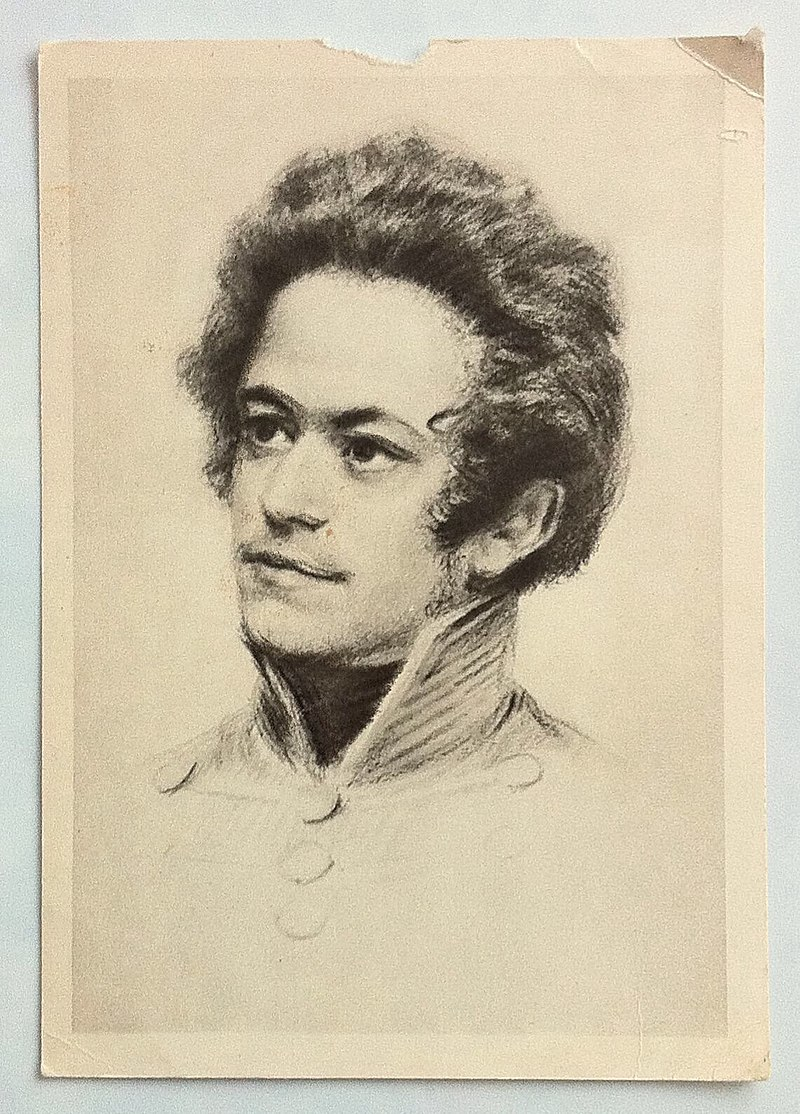
\includegraphics[width=\onequartertextwidth]{../resources/sample-image.png}
	\caption{\textbf{Figure \ref{fig:sample}.} \textit{A sample image}}
	\label{fig:sample}
\end{figure}

\\
And tables:
\begin{table}[H]
	\centering
	\caption{\textbf{Table \ref{tab:sample}.} \textit{A sample table}}
	\begin{tabular}{|c|c|}
		\hline
		C & D \\ \hline
		3 & 4 \\ \hline
	\end{tabular}
	\label{tab:sample}
\end{table}

And you can reference them: Figure~\ref{fig:sample}, Table~\ref{tab:sample}.

Note that if you need to repeat a citation, I recommend using \textit{refcite} command provided by this tool, as in \refcite{einstein2013principle}.

% bibliography can be added
\bibliography{../resources/Bibliography}
